\documentclass[a4paper,12pt]{article}

\title{Chemistry 30 IB \\ Acids \& Bases}
\author{Jad Chehimi}

% document setup
\renewcommand{\familydefault}{\sfdefault}
\linespread{1.25}
\usepackage{setspace}
\usepackage{enumitem}
\setlist{nosep}

% tools
\usepackage{siunitx}
\usepackage[version=4]{mhchem}
\usepackage[hidelinks]{hyperref}
\usepackage{float}
%% images
\usepackage{graphicx}
\graphicspath{ {./images/} }

\usepackage[margin=1in]{geometry}

\begin{document}
\maketitle

% temp
\begin{center}
\Huge
Unfinished!
\normalsize
\end{center}
% temp

\tableofcontents

\pagebreak

\section{Theories}
The following two equations mean the same thing.

\ce{H+(aq)} and \ce{H3O+(aq)} are interchangable.

\subsection{Arrhenius}
\Large
$$\ce{HX(aq) -> H+(aq) + X-(aq)}$$
\normalsize
\begin{itemize}
    \item{doesn't specifically state water is present (aq)}
    \item{uses hydrogen ions, \ce{H+(aq)}}
    \item{cannot determine strong or weak}
\end{itemize}

\subsection{Br{\o}nsted-Lowry (aka. Modified Arrhenius)}
\Large
$$\ce{HX(aq) + H2O(l) -> H3O+(aq) + X-(aq)}$$
\normalsize
\begin{itemize}
    \item{specifically states water is present}
    \item{uses hydronium ions, \ce{H3O+(aq)}}
    \item{can determine strong or weak}
\end{itemize}

\section{General Equations}

\begin{itemize}
    \item{Chemical entities not present in the data booklet pages 8-9---such as \ce{K+}, \ce{Mg{2+}}, \ce{Na+}, \ce{Cl-}---are spectators and do not need to be included in the equations.}
    \item{Chemical entities from the first six rows in the data booklet pages 8-9---such as \ce{ClO4-}---do not need to be included in equations, as equations containing said entities ionize/dissociate completely, leaving the hydronium/hydroxide ions by themselves.}
\end{itemize}

\subsection{Ionization of Acids}
Forming ions from molecular compounds.

\subsubsection{Strong}
\Large
$$\ce{HX(aq) + H2O(l) ->[$>99.9\%$] H3O+(aq) + X-(aq)}$$
\normalsize
\begin{itemize}
    \item{ionize completely ($>99.9\%$ of the reaction completes)}
    \item{irreversible (\ce{->})}
    \item{high $K$ value ($K > 1$)}
\end{itemize}

\subsubsection{Weak}
\Large
$$\ce{HX(aq) + H2O(l) <=>[$<50\%$] H3O+(aq) + X-(aq)}$$
\normalsize
\begin{itemize}
    \item{do not ionize completely ($<50\%$ of the reaction completes)}
    \item{reversible (\ce{<=>})}
    \item{ionize at equilibrium}
    \item{low $K$ value ($K < 1$)}
\end{itemize}

\subsection{Dissociation of Bases}
Separation of existing ions in solution.

\subsubsection{Strong}
\Large
$$\ce{M(OH)_n + H2O(l) ->[$>99.9\%$] M^{n+}(aq) + nOH-(aq)}$$
\normalsize
\begin{itemize}
    \item{\ce{M} is a metal, \ce{M(OH)_n} is highly soluble}
    \item{dissociate quantitatively}
\end{itemize}

\subsubsection{Weak}
\Large
$$\ce{X(aq) + H2O(l) <=>[$<50\%$] HX+(aq) + OH-(aq)}$$
\normalsize
\begin{itemize}
    \item{dissociate at equilibrium}
\end{itemize}

\section{pH \& pOH}
\subsection{pH/pOH from Concentration}
\Large
$$\textrm{pH} = -\log{[\ce{H3O+}]}$$
$$\textrm{pOH} = -\log{[\ce{OH-}]}$$
\normalsize

\subsubsection{Shortcut}
The absolute value of the exponent of a concentration is the pH/pOH, for hydronium and hydroxide concentrations respectively.

e.g. $\SI{1.00e-4}{\mol\per\L}$ of \ce{H3O+} has a $\textrm{pH} = 4$

\subsection{Estimation}
This isn't required to know.

This only applies if the base is equal to 1.00. If the base is not 1.00, you can predict ranges that the pH/pOH could be. 

Of course, you can just calculate it, but this is a trick you can use to quickly figure out and compare pH/pOH from concentration.

\begin{itemize}
    \item{If $[\;\;] = 1$, then $\textrm{pH} = |exponent|$}
    \item{If $[\;\;] > 1$, then $\textrm{pH} < |exponent|$}
    \item{If $[\;\;] < 1$, then $\textrm{pH} > |exponent|$}
\end{itemize}


\subsection{Concentration from pH/pOH}
\Large
$$[\ce{H3O+}] = 10^{-\textrm{pH}}$$
$$[\ce{OH-}] = 10^{-\textrm{pOH}}$$
\normalsize

\subsection{Switching between pH and pOH}
\Large
$$\textrm{pH} + \textrm{pOH} = 14$$
\normalsize

\subsection{$K_w$}
The equilibrium constant of water can be used to solve for hydrogen ion concentration or hydronium ion concentration when you have the other.

$$K_w = [\ce{H3O+}][\ce{OH-}]$$

$$K_w = \SI{1.00e-14}{\mol\per\L}$$

$$\SI{1.00e-14}{\mol\per\L} = [\ce{H3O+}][\ce{OH-}]$$

\subsection{Significant Digits}
The significant digits of the concentration is the number of decimal pleaces of the pH/pOH.

For instance,
\begin{figure}[H]
    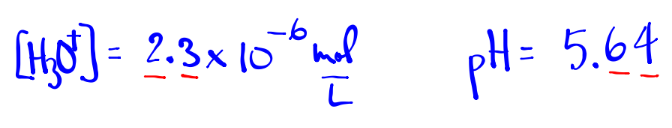
\includegraphics[width=\textwidth]{ph-sigdigs}
\end{figure}

\subsection{Square}
This may help you remember when to use what.
\begin{figure}[H]
    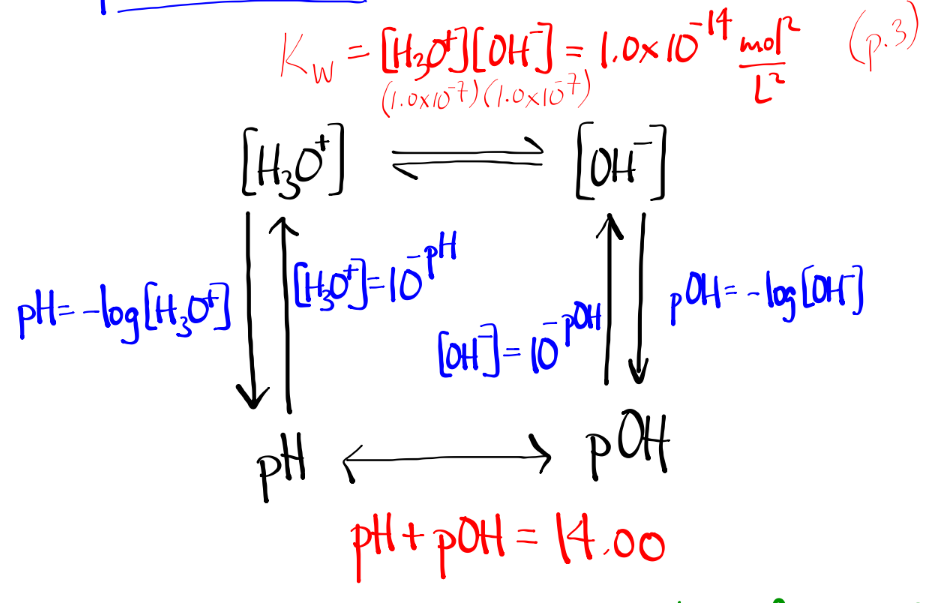
\includegraphics[width=\textwidth]{ph-square}
\end{figure}

\subsection{Example}
\begin{figure}[H]
    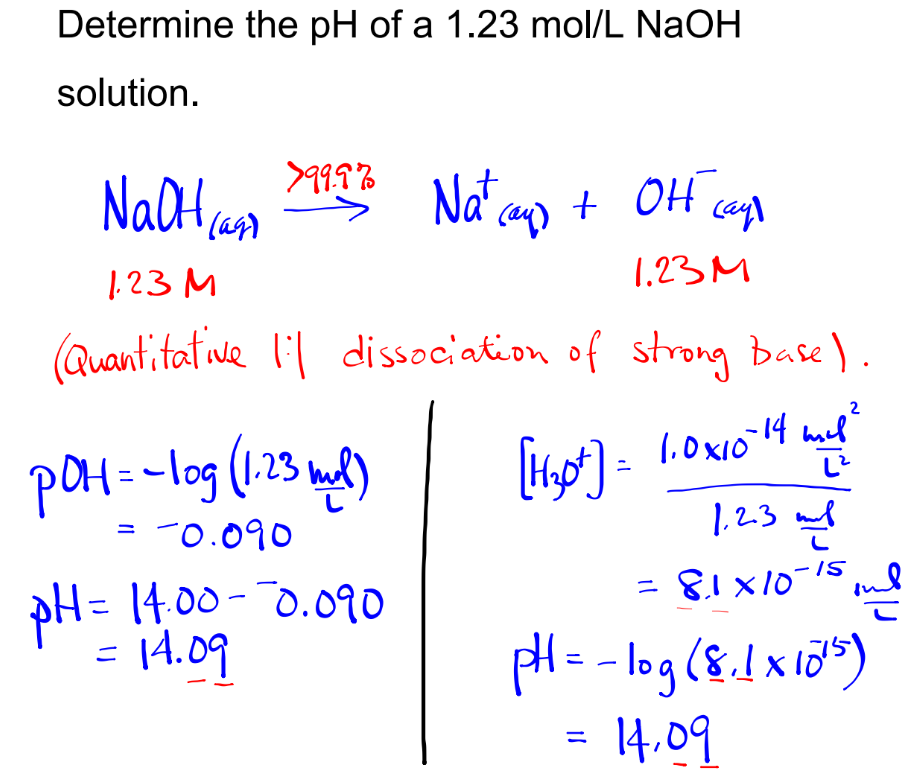
\includegraphics[width=\textwidth]{ph-example}
\end{figure}

\section{Acid/Base Reaction}
Also known as a neutralization reaction.

The complete or partial transfer of protons (\ce{H+}) from the strongest acid to the strongest base. The acids donate protons, the bases accept protons.

\normalsize
\begin{figure}[H]
    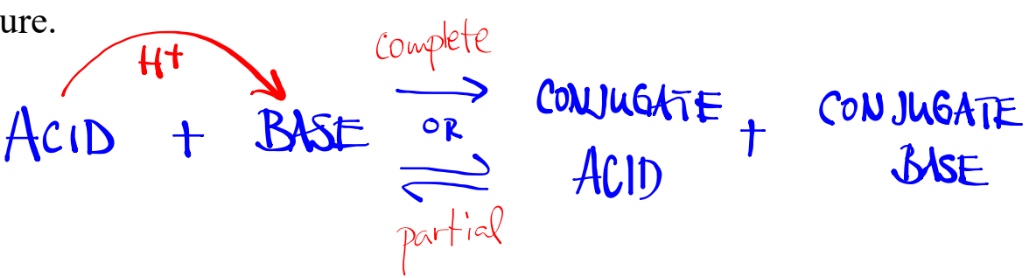
\includegraphics[width=\textwidth]{acidbase}
\end{figure}

\subsection{Net Reaction}
At this level, we typically only see the net reaction.

For your information, this is what leads to the net reaction.
\begin{figure}[H]
    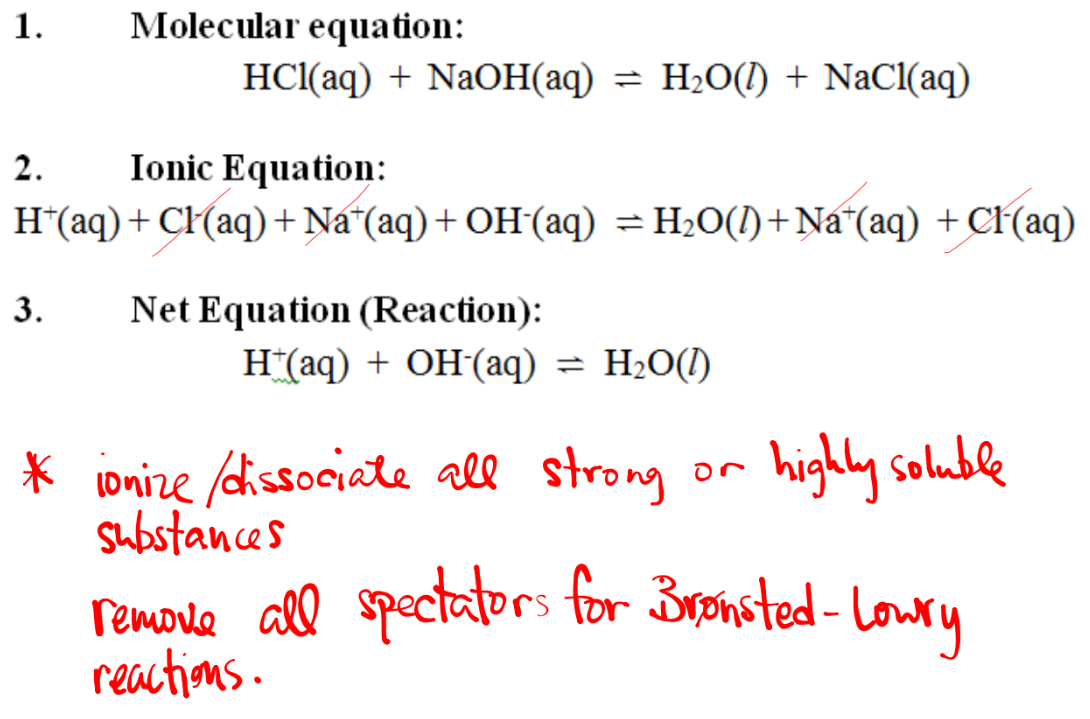
\includegraphics[width=\textwidth]{net}
\end{figure}

\subsection{Example Net Reactions}
\begin{figure}[H]
    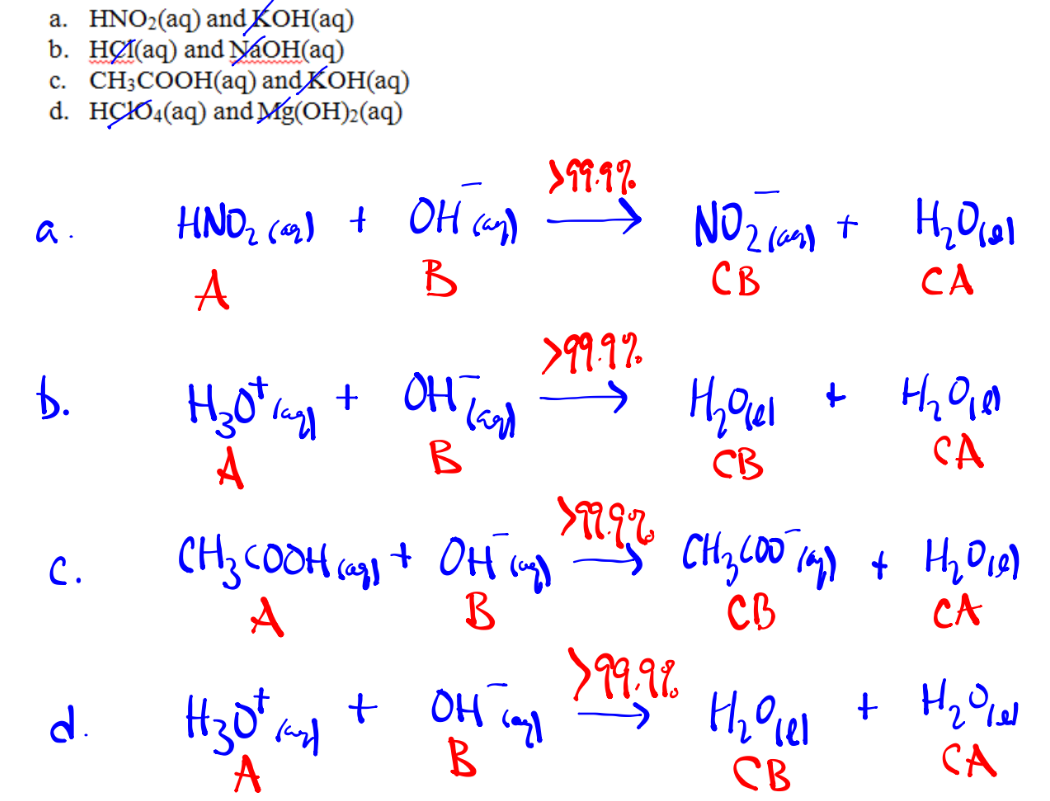
\includegraphics[width=\textwidth]{equationex}
\end{figure}

\subsection{Conjugate}
\begin{itemize}
    \item{The conjugate base (CB) is what an acid becomes on the product side.}
    \item{The conjugate acid (CA) is what a base becomes on the product side.}
\end{itemize}

Conjugates differ from their original by one proton. (\ce{H+})

This is because, say a compound loses a proton from left to right, then it is an acid. Read that in reverse, right to left, and it gains a proton, making it a base.
\begin{figure}[H]
    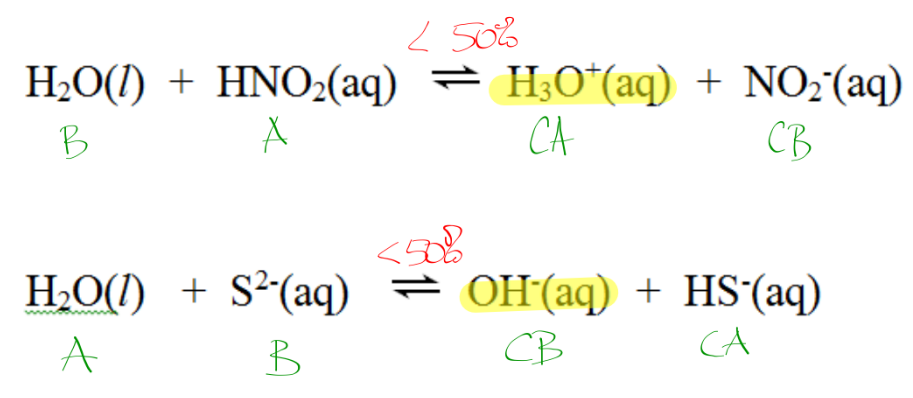
\includegraphics[width=\textwidth]{conjugate}
\end{figure}

A conjugate pair would be either,
\begin{itemize}
    \item{an acid and its conjugate base}
    \item{a base and its conjugate acid}
\end{itemize}

\subsection{Polyprotic Acids}
Acids that can donate a proton more than once.

They do it one at a time, yielding a different $K_a$ value every time.

\begin{itemize}
    \item{$\ce{H2CO3(aq) + H2O(l) <=> H3O+(aq) + HCO3-(aq)} \;\;\;\;\;\; K_a = \num{4.4e-7}$}
    \item{$\ce{HCO3-(aq) + H2O(l) <=> H3O+(aq) + CO3^{2-}(aq)} \,\;\;\;\;\;\; K_a = \num{4.7e-11}$}
\end{itemize}

For calculating the pH of a polyprotic acid, the $K_a$ of the first ionization should be used for calculations.

The conjugate base of polyprotic acids are amphiprotic.

\subsection{Amphiprotic}
Sometimes called amphoteric. Water is amphiprotic.

Substances that are both a base and an acid. Whether they behave as an acid or a base depends on the other substance in the acid/base reaction. 

It will do the opposite of the other substance, so if it were an acid, the amphiprotic will behave as a base, and vice versa.

Amphiprotics also often are a negative ion with hydrogen---\ce{HX-}---such as \ce{HSO4-(aq)}.

If both substances in an acid/base reaction can behave as an acid, the stronger acid will behave as an acid, the other as a base.

\subsection{Favourability}
\subsubsection{Hydronium or Hydroxide Present}
If \ce{H3O+} or \ce{OH-} are present, the reaction will favour the side they are not on.

If either one of these two ions are,
\begin{itemize}
    \item{a reactant, then products are favored. \ce{->[$>99.9\%$]}}
    \item{a product, then reactants are favored. \ce{<=>[$<50\%$]}}
\end{itemize}

\subsubsection{No Hydronium/Hydroxide}
On page 8-9 in your data booklet,
\begin{itemize}
    \item{if the acid is above the base, then products are favored. \ce{->[$>99.9\%$]}}
    \item{if the base is above the acid, then reactants are favored. \ce{<=>[$<50\%$]}}
\end{itemize}

The higher on the table, the stronger the acid. If the acid is stronger, it'll more likely donate protons, increasing the concentration of the opposing side of the reaction.

\section{(AB) Relative Strength}
The following is, oddly enough, non-IB.

\begin{itemize}
    \item{$K_a$ = acid equilibrium constant \\ how much \ce{H3O+(aq)} is produced when an acid interacts with water}
    \item{$K_b$ = base equilibrium constant \\ how much \ce{OH-(aq)} is produced when an base interacts with water}
\end{itemize}

Equilibrium constants are calculated the same as usual. Product of concentrations of products divided by product of concentrations of reactants, not including liquid water.

\subsection{$K_a$ of Common Substances}
The equilibrium constant of many common acids is provided on page 8-9 of the Alberta data booklet, on the right-most column.

But what if you want $K_b$?

\subsection{Converting between acid/base equilibrium constants}
\Large
$$K_w = K_a \times K_b$$
\normalsize

This means you can calculate $K_b$ as long as you have $K_a$, since $K_w$ is a known constant.

The $K_a$ of a base on the table is actually the conjugate acid. Doesn't really change anything---they are on the same line, after all---but good to know.

\Large
$$K_b = \frac{\SI{1.0e-14}{\mol\per\L}}{K_a}$$
\normalsize

If the $K_b > K_a$, than the base is a stronger base than the conjugate is an acid. This doesn't always mean its a base---its just a stronger base.

\subsubsection{Example}
The target base is ammonia, \ce{NH3}. The conjugate acid of ammonia, ammonium \ce{NH4+}, has a $K_a$ listed on the table---\SI{5.6e-10}{\mol\per\L}.

Therefore,
$$K_b = \frac{\SI{1.0e-14}{\mol\per\L}}{\SI{5.6e-10}{\mol\per\L}}$$
$$K_b = \SI{1.7e-5}{\mol\per\L}$$
Ammonia \ce{NH3} is a stronger base than ammonium \ce{NH4+} is an acid.

\section{pH/pOH and Ion Concentration of Weak Acids/Bases}
\subsection{Strong}
Strong acids and bases ionize/dissociate completely, respectively. The concentrations of the acid/base is equal to the concentration of hydronium/hydroxide ions. They ionize/dissociate quantitatively.

\begin{center}
    $[\textrm{acid}] = [\ce{H3O+}]$ \hspace{1in} $[\textrm{base}] = [\ce{OH-}]$
\end{center}

\subsection{Weak}
If you want the full explanation of where these formulas are derived from, read the actual notes---page 38. The following are the shortcuts you truly only need.

\subsubsection{Known Ion Concentration}
The following should be used if you know the ion concentration or pH/pOH, since pH/pOH can be converted into ion concentration.

\begin{center}
\Large
$K_a = \frac{[\ce{H3O+}]^2}{[\textrm{acid}] - [\ce{H3O+]}}$
\hspace{0.5in}
$K_b = \frac{[\ce{OH-}]^2}{[\textrm{base}] - [\ce{OH-]}}$
\normalsize
\end{center}

\subsubsection{Unknown Ion Concentration}
If you are solving for ion concentration with the aforementioned formula, you will require the quadratic formula. To avoid this, the ion concentration in the denominator can be omitted, since it affects the calculation negligably.

\begin{center}
\Large
$K_a = \frac{[\ce{H3O+}]^2}{[\textrm{acid}]}$
\hspace{0.5in}
$K_b = \frac{[\ce{OH-}]^2}{[\textrm{base}]}$
\normalsize
\end{center}

Therefore, you can now find ion concentration of weak acids/bases.

\begin{center}
\Large
$[\ce{H3O+}] = \sqrt{K_a \cdot [\textrm{acid}]}$
\hspace{0.5in}
$[\ce{OH-}] = \sqrt{K_b \cdot [\textrm{base}]}$
\normalsize
\end{center}

\pagebreak

\section{Acid Base Titrations}

Titration is a method for measuring the concentration of a solution.

The \textbf{titrant} is the solution in the burette, typically just an acid or base.

The \textbf{sample} is the solution in the Erlenmeyer flask, typically composed of a solution and an indicator. The indicator can be used to determine the pH of the solution after titrating the titrant.

\textbf{Indicators} are given to you on page 10 of the data booklet. Each column has the acid variant on the left and base variant on the right. For instance, bromothymol blue is yellow below 6.0 pH, blue above 7.6 pH, and green in between (indicating the equivalence point).

\begin{figure}[H]
    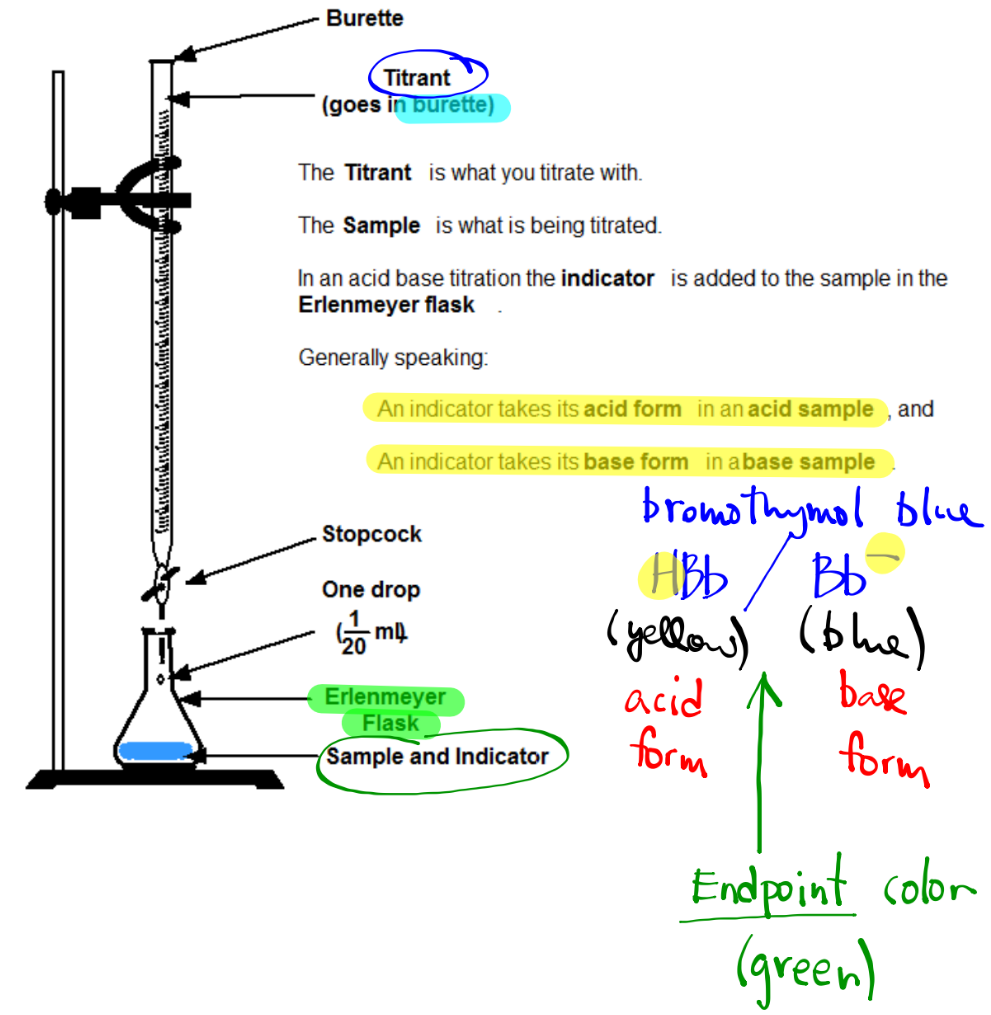
\includegraphics[width=\textwidth]{titration}
\end{figure}

\section{Equivalence Point}
\begin{itemize}
    \item{Adding base to an acid neutralizes it, \ce{[ H+ ]} decreases while \ce{[ OH- ]} increases.}
    \item{Adding acid to an base neutralizes it, \ce{[ H+ ]} increases while \ce{[ OH- ]} decreases.}
\end{itemize}

Eventually, \ce{[ H+ ] = [ OH- ]}.

This is the equivalence point---when a proton is quantitatively exchanged completely. It shows up as the half way point in a steep jump/drop on neutralization graphs.

\begin{itemize}
    \item{The pH at the equivalence point is the pH of neutralization.}
    \item{The volume at the equivalence point is the volume of titrant needed to be titrated/added to neutralize sample.}
\end{itemize}

\subsection{Example Problem}
It is just stoicheometry.

\SI{10.0}{\mL} of an unknown concentration of \ce{NaOH} is placed in a flask. A drop of indicator is added. A \SI{2.00}{\mol\per\L} solution of \ce{HCl} is added until a colour change occurs. If it takes \SI{25.0}{\mL} of \ce{HCl} to reach the equivalence point, what is the concentration of the \ce{NaOH}?

(\ce{Cl} and \ce{Na} are spectators.)

$$\ce{H+(aq) + OH-(aq) <=> H2O(l)}$$

$$\SI{0.25}{\L}\;\ce{HCl} \times \frac{\SI{2.00}{\mol}\;\ce{HCl}}{\SI{1}{\L}\;\ce{HCl}} \times \frac{\SI{1}{\mol}\;\ce{NaOH}}{\SI{1}{\mol}\;\ce{HCl}} \times \frac{1}{\SI{0.0100}{\L}\;\ce{NaOH}}$$

$$=\SI{5.00}{\mol\per\L}\;\ce{NaOH(aq)}$$

\subsection{Example Problem 2}
\begin{figure}[H]
    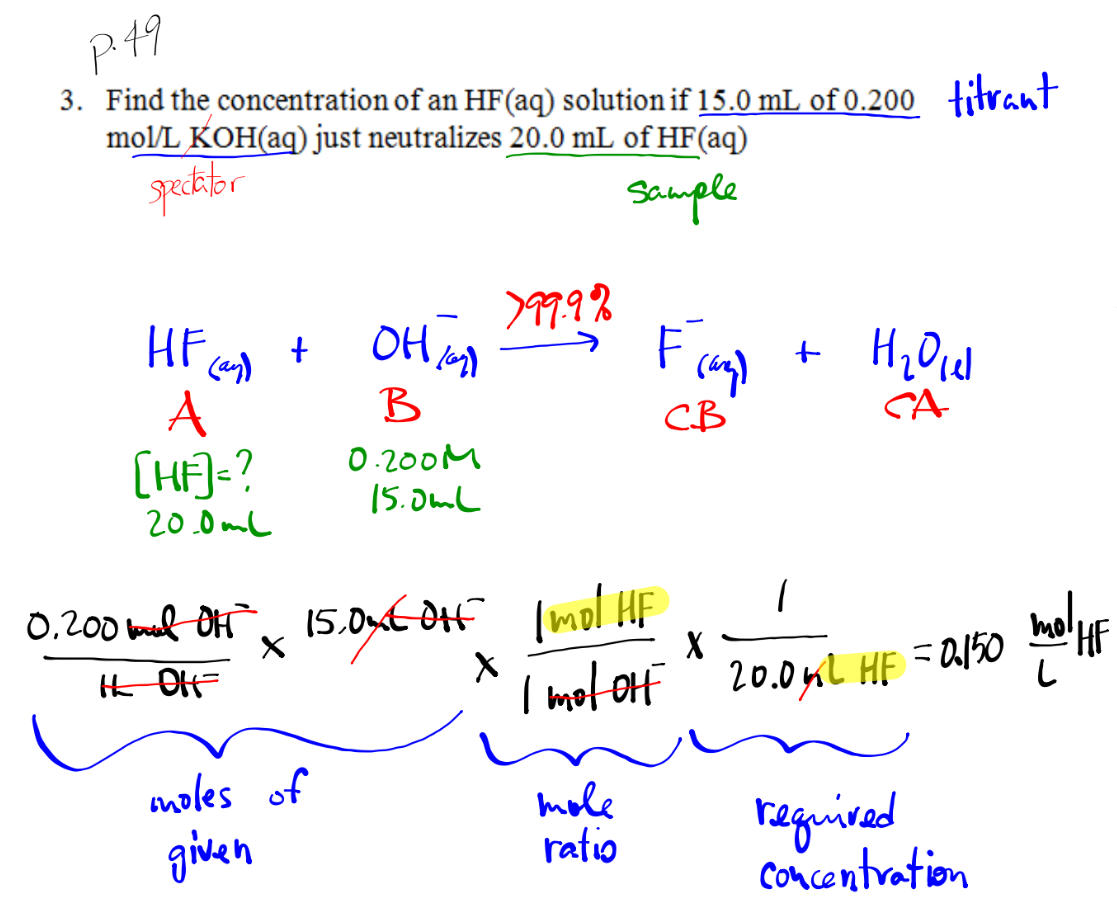
\includegraphics[width=\textwidth]{equivex}
\end{figure}


\section{Neutralization Reactions Graphs}
\begin{itemize}
    \item{A large jump/drop in the graph signifies an equivalence point}
    \item{The number of equivalence points = the number of protons transferred}
    \item{Proton exchange reactions that are at equilibrium do not result in large changes in pH}
\end{itemize}

\subsection{Strong Acid \& Strong Base}
\begin{figure}[H]
    \centering
    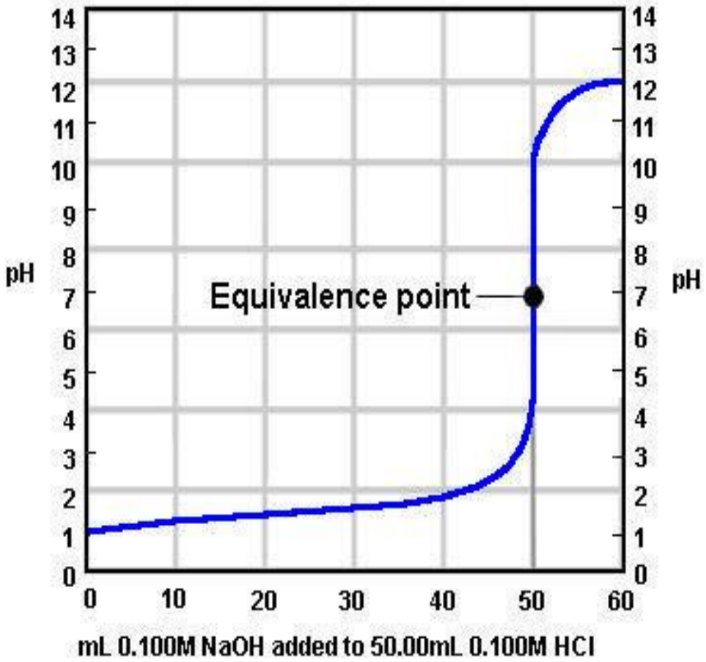
\includegraphics[width=0.9\textwidth]{strongacid-strongbase}
    \caption{The line is both the acid and base pH, which are equal}
\end{figure}
Acidic sample---as pH starts low. Basic titrant---as pH ends high. A basic sample and acidic sample would be this graph reversed.

Equivalence point is always $= 7$.

\textbf{Explanation}
\begin{itemize}
    \item{pH increases slowly at first, as it initially takes a lot of acidic hydroxide ions to remove basic hydronium ions}
    \item{Once there are very little acidic ions, not a lot of basic ions are needed to increase the pH}
    \item{Therefore, the pH jumps very rapidly}
    \item{Since the acidic hydronium ion concentration is low, it will again take a lot of base to increase the hydroxide ion concentration}
\end{itemize}

\subsection{Strong Base \& Weak Acid}
\begin{figure}[H]
    \centering
    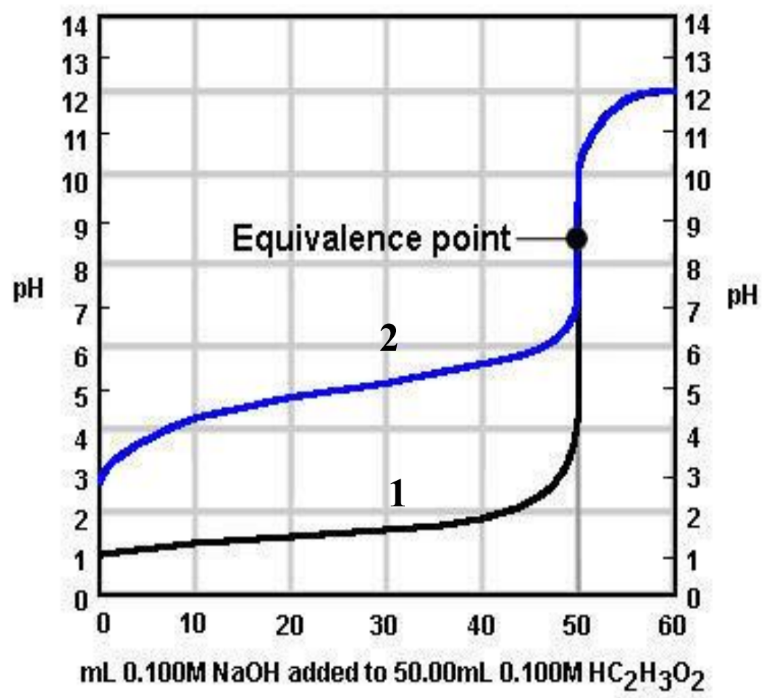
\includegraphics[width=0.9\textwidth]{strongbase-weakacid}
    \caption{Line 1 (black) is strong base / Line 2 (blue) is weak acid}
\end{figure}

Equivalence point is always $> 7$.

\textbf{Weak Acid (Line 2) Differences}
\begin{itemize}
    \item{Starts with a higher pH than the strong acid (line 1)}
    \item{Brief curve up at beginning (from 0-10 mL) before linear slope}
    \item{Region between brief curve and equivalence point (from 10-45 mL) is \textbf{buffer}}
\end{itemize}

\subsection{Strong Acid \& Weak Base}
\begin{figure}[H]
    \centering
    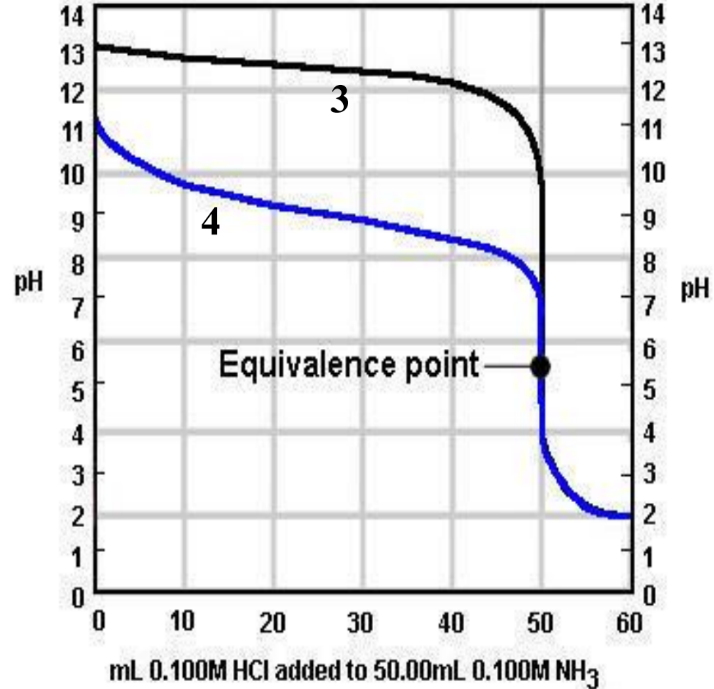
\includegraphics[width=0.9\textwidth]{strongacid-weakbase}
    \caption{Line 3 (black) is strong acid / Line 4 (blue) is weak base}
\end{figure}

Equivalence point is always $< 7$.

\begin{itemize}
    \item{Starts with a lower pH than the strong base (line 3)}
    \item{Brief curve down at beginning (from 0-10 mL) before linear slope}
    \item{Region between brief curve and equivalence point (from 10-45 mL) is \textbf{buffer}}
\end{itemize}

\subsection{Polyprotic Acid Titrations}
\begin{figure}[H]
    \centering
    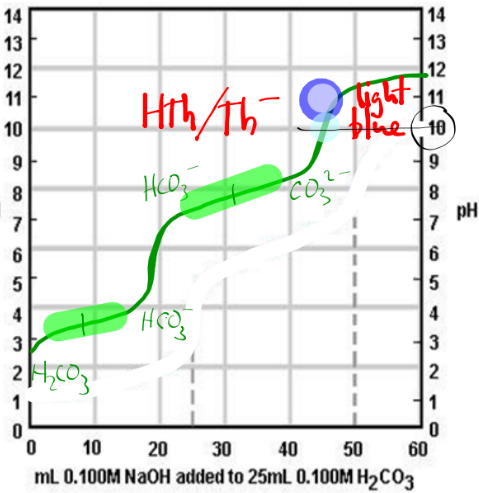
\includegraphics[width=0.9\textwidth]{polyprotic}
\end{figure}
\begin{itemize}
    \item{Multiple jumps in line (multiple equivalence points)}
    \item{Flat regions between equivalence points (highlighted green) are buffers}
    \item{Last flat region is not a buffer}
    \item{Jumps after the first one are not as large}
\end{itemize}

\pagebreak

\section{Buffers}
Buffers are equal molar concentrations of a weak acid and its weak conjugate base. 

A buffer resists changes in pH when small amounts of \ce{H3O+(aq)} or \ce{OH-(aq)} are added to them. In other words, they absorb small additions of acids or bases, converting them into weaker forms.

\subsection{Composition}
Buffers are comprised of two components---a weak base and a weak acid in equal molar concentrations.

The weak base and weak acids will be conjugates of each other. For example,
\begin{itemize}
    \item{\ce{CH3COOH(aq) / CH3COO-(aq)}}
    \item{\ce{H2PO4^-(aq) / HPO4^{2-}(aq)}}
    \item{\ce{H2CO3(aq) / HCO3-(aq)}}
    \item{Generically, \ce{HA(aq) / A-(aq)}}
\end{itemize}

\subsection{Adding \ce{H3O+(aq)} To A Buffer}
$$\ce{weak base + H3O+(aq) <=> weak conjugate acid + H2O(l)}$$
\begin{itemize}
    \item{Buffer reacts with hydronium ions (\ce{H3O+(aq)})}
    \item{Produces water (neutral pH)}
    \item{Produces conjugate acid of weak base (very weak, pH decreases slightly)}
\end{itemize}

\subsection{Adding \ce{OH-(aq)} To A Buffer}
$$\ce{weak acid + OH-(aq) <=> weak conjugate base + H2O(l)}$$
\begin{itemize}
    \item{Buffer reacts with hydroxide ions (\ce{OH-(aq)})}
    \item{Produces water (neutral pH)}
    \item{Produces conjugate base of weak acid (very weak, pH increases slightly)}
\end{itemize}

\subsection{Ideal Conditions}
Buffers work best if...
\begin{itemize}
    \item{strength of acid and base are equal}
    \item{concentration of acid and base are equal}
\end{itemize}

\subsection{Consumption}
Once the weak acid or base is consumed---called the buffering capacity---there will be a rapid change in pH.

\subsection{Application}
You may be asked to find which pH a buffer is most effective.

$$\ce{HA(aq) + H2O(l) <=> A-(aq) + H3O+(aq)}$$

Since the concentration of the acid and the conjugate base are equal in a buffer, they cancel in a $K_a$ expression.

$$K_a = \frac{[\ce{H3O+}][\ce{A-}]}{[\ce{HA}]}$$

$$K_a = [\ce{H3O+}]$$

Since the $K_a$ is just the hydronium ion concentration, getting the negative log of it will give you the effective pH for the buffer.

Essentially, the following is true.

$$\textrm{ideal buffer pH} = -\log{K_a}$$

\subsection{Visualization}
\begin{figure}[H]
    \centering
    \caption{The buffering regions are denoted as boxed areas in the following graphs}
    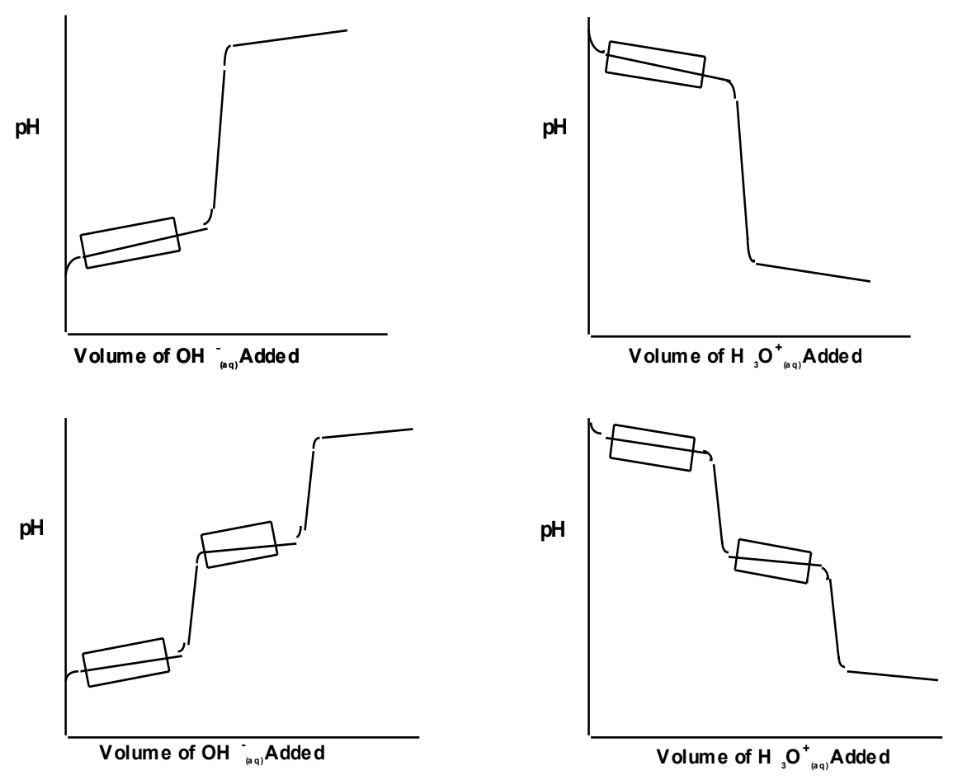
\includegraphics[width=\textwidth]{buffers}
\end{figure}
\begin{itemize}
    \item{Buffer regions are typically before and in between equivalent points}
    \item{There are no buffer regions in titrations of strong acids and strong bases}
    \item{The region following the final equivalence point is not a buffer region. Rather, strong acids or bases are being added to a solution already dominated by strong acids or bases respectively. Therefore, there isn't a significant pH change}
\end{itemize}

\end{document}
